 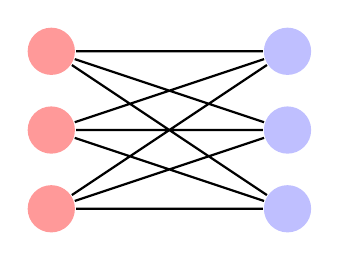
\begin{tikzpicture}[auto,thick,every node/.style={circle, minimum size=0.6cm,fill=blue!25}]
 	\node (p0) [fill=red!40]{};
 	\node (p1) [below of=p0, fill=red!40] {};
 	\node (p2) [below of=p1, fill=red!40] {};
 	\node (p3) [right of=p2,xshift=2cm] {};
 	\node (p4) [above of=p3] {};
 	\node (p5) [above of=p4] {};

 	\draw       
 	(p0) -- (p3)
 	(p0) -- (p4)
 	(p1) -- (p3)
 	(p1) -- (p4)
 	(p2) -- (p3)
 	(p2) -- (p4)
 	(p5) -- (p0)
 	(p5) -- (p1) 
 	(p5) -- (p2);    
 \end{tikzpicture}                
